\documentclass{article}

% Language setting
% Replace `english' with e.g. `spanish' to change the document language
\usepackage[english]{babel}
\usepackage{float}

% Set page size and margins
% Replace `letterpaper' with `a4paper' for UK/EU standard size
\usepackage[letterpaper,top=2cm,bottom=2cm,left=3cm,right=3cm,marginparwidth=1.75cm]{geometry}

% Useful packages
\usepackage{amsmath}
\usepackage{graphicx}
\graphicspath{{images/}}
\usepackage[colorlinks=true, allcolors=blue]{hyperref}

\title{Midterm Checkpoint Report}
\author{Chenfeng Li, Qian Liu, Nathan Suhr}

\begin{document}
\maketitle

\section{Introduction}

Our project is an agent-based model for tracking an illness in a population. In this simulation, a number of people (specified by the user) are put onto a grid and move on this grid during each time step. If any uninfected person comes in proximity of an infected one, they will have a chance to become infected as well. Currently, our simulation tracks the number of people infected, dead, recovered, and healthy during each time step. This information is then plotted and is the main output for our data. \\The focus of our project is maintaining performance while implementing features that would contribute to the realism of our model. To aid this, we plan on implementing the use of data from real pandemics such as transmission rate depending on proximity and chance of infection depending on mask usage. However, we plan on having some of these parameters able to be set by our user, which would lead to our model being versatile, and applicable to many situations. \\The primary question we hope to answer from the results of our data is how the initial parameters affect the convergence of the model. The convergence of this model is extremely insightful for those hoping to assess a disease's potential impact on a population over time. Once this occurs, this could imply that the population has reached herd immunity or that the main impact of the disease has run its course. Additionally, by analyzing infection rate with given parameters, one can see how quickly an illness will spread and this information could help officials prepare for these effects.

\section{Numerical Methods and Packages}

In order to record that status for people on each time step, we use deepcopy from the copy package. We create a deepcopy of a list as opposed to a shallow one specifically to avoid using pointers or references. This way, when we append the status after each time step, we will not risk altering the statuses we have previously appended. \\Additionally, we plan on using the interp1d package as well as other interpolators. These will be used to approximate functions for each of the four curves that are plotted. This way, without running our actual model, we can simulate the data for much larger amounts of time steps. 

\section{Structuring of src}

Currently, our code is formatted such that the user only needs to change the parameters of one function that runs the entire simulation. Due to this, we will put one file into the src folder. If the user wants to run the code, they must import Disease\_Model\_Source\_Code, and then use their virus function to create a virus of the user's liking. After this, the user must run the simulation function (with the function parameters changed to the user's liking), the entire simulation will run and the user can see the plot by running sim.plot(), can see all the boards by using sim.record, and can see the animation by using sim.animate(). Examples of how to do this process can be seen in the examples folder.

\section{Tests}

We have multiple tests for both the person class and the simulation class as of now. For the person class, we have three tests. One tests whether a person is constructed and initialized correctly. Another tests whether the status of a person object can be changed correctly. The last one tests whether a person can move on the board correctly. We also have tests for the simulation. These test whether the simulation is initialized correctly, whether people move correctly in the simulation, and whether the infection spreads. In particular, the movement test ensures nobody moves out of the bounds of the board and that no two people are overlapping. \\ Our code currently passes five tests and fails the test for the infection in the simulation. For that test, our goal is to have an extreme case that there is one infected person at the beginning and two infected people at the end. We will look into it further to debug the error.

\section{Results}
We ran six simulations for our model with the same setting for the properties of the virus. We set the probability of a healthy person being infected by a carrier as $\frac{1}{10}*distance^2$, the probability of an infected person carrying the virus to the next time step as 0.95, and the fatality rate as 10%. Upon running six trials for our model, we found that the information derived from examining the plot was reasonable. 
\begin{figure}[H]
    \centering
    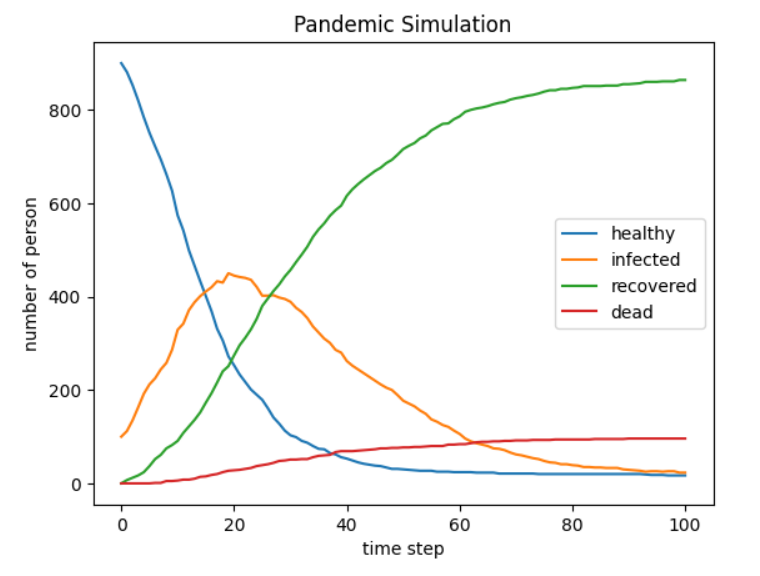
\includegraphics[width=.6\linewidth]{situation1.png}
    \caption{100 * 100 board with 1000 people, (10\% infected), 100 time steps}
    \label{fig:enter-label}
\end{figure} 
From figure 1, we find that all four types of people seem to converge. The number of healthy, infected, dead, and recovered seems to plateau which implies that everyone infected has either died or recovered. This hypothesis is complemented by noting that the amount of healthy people is zero at the end of the simulation. Since people cannot be infected more than once at this point, these results make sense. All the lines are monotone aside from the amount of people infected which also makes sense. People cannot die and come back to life, nor can they get infected twice or return to healthy status after infection. \\
\begin{figure}[H]
    \centering
    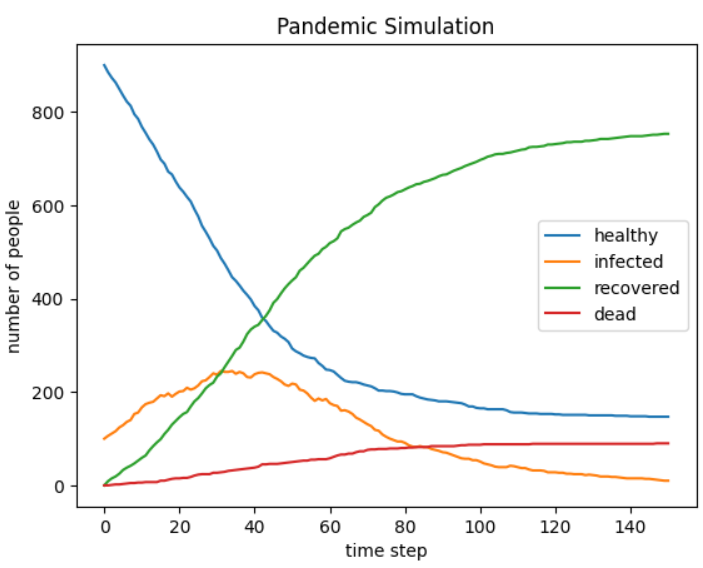
\includegraphics[width=.6\linewidth]{situation2.PNG}
    \caption{150 * 150 board with 1000 people, (10\% infected), 150 time steps}
    \label{fig:enter-label}
\end{figure}
The plots for figure 2 and 1 initially look similar. However, all the lines are less steep in figure 2 and there are 1.5x as many time steps. Because the board size is much larger in figure 2, it will take longer for the infection to spread since people are spaced further apart. Thus, the infection curve being wider makes sense. So too do the steepness of the healthy and recovered curves. \\
\begin{figure}[H]
    \centering
    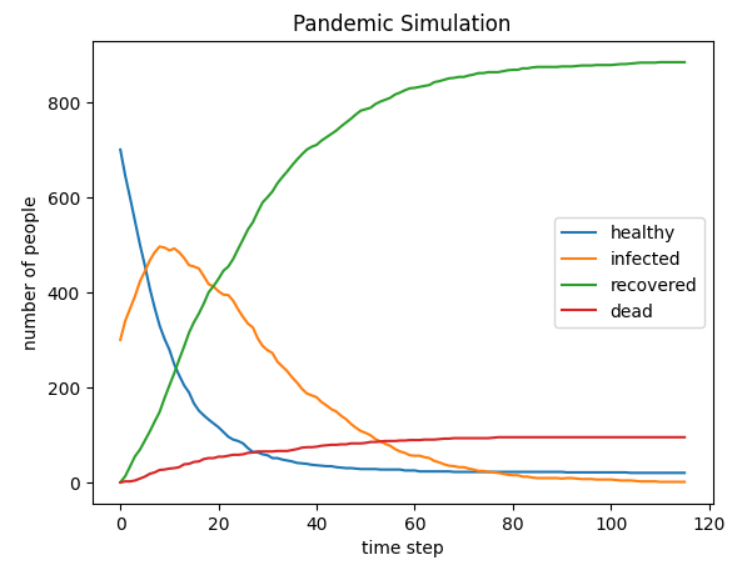
\includegraphics[width=.6\linewidth]{situation3.PNG}
    \caption{100 * 100 board with 1000 people, (30\% infected), 115 time steps}
    \label{fig:enter-label}
\end{figure}
From figure 3, we can see that our model correctly accounts for a higher number of people initially affected. This can be seen from the starting positions of the infected and healthy curves. Additionally, we can see that the infection rate plateaus quicker because the higher initial infection rate led to the disease spreading faster than the other scenarios. \\
\begin{figure}[H]
    \centering
    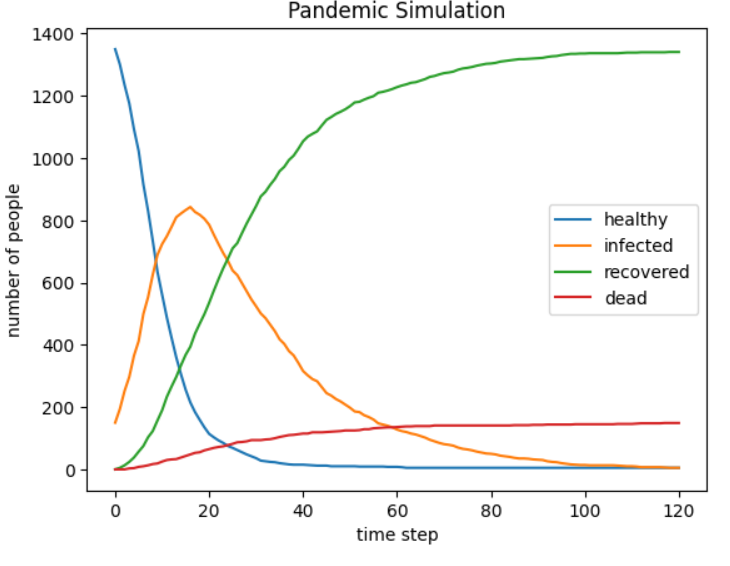
\includegraphics[width=.6\linewidth]{situation4.PNG}
    \caption{100 * 100 board with 1500 people, (10\% infected), 120 time steps}
    \label{fig:enter-label}
\end{figure}
\begin{figure}[H]
    \centering
    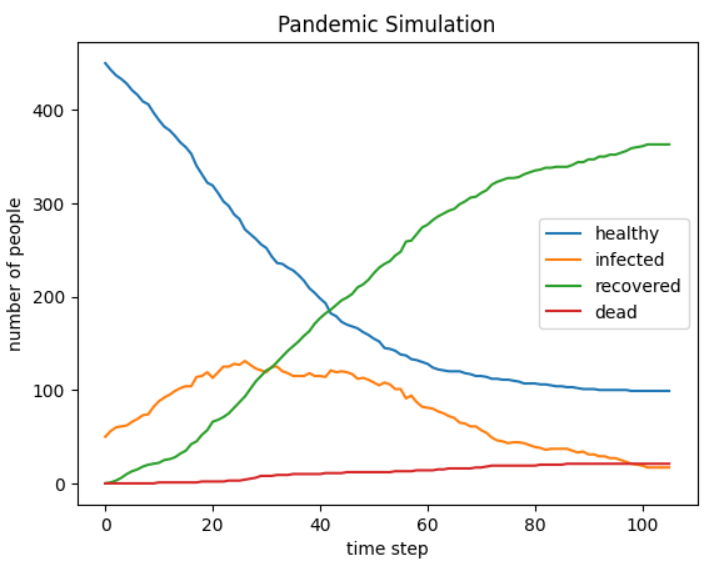
\includegraphics[width=.6\linewidth]{situation5.PNG}
    \caption{100 * 100 board with 500 people, (10\% infected), 105 time steps}
    \label{fig:enter-label}
\end{figure} 
We can see from figure 4 that concentrating more people on a board will yield higher infection rates, quicker infection plateaus, and a much steeper descent on the curve of healthy people. This is reasonable since, due to the area being smaller and people interacting more often, the disease will propagate faster. The opposite occurrence can be seen in figure 5, which is almost identical to figure 4 except with a third the amount of people. Due to less people inhabiting a space of equal size, there is a decreased likelihood of interaction and disease propagation. The effects of this are clearly visible on the plot of figure 5. All of the curves are much flatter, especially the infected curve which has a much wider plateau. \\
\begin{figure}[H]
    \centering
    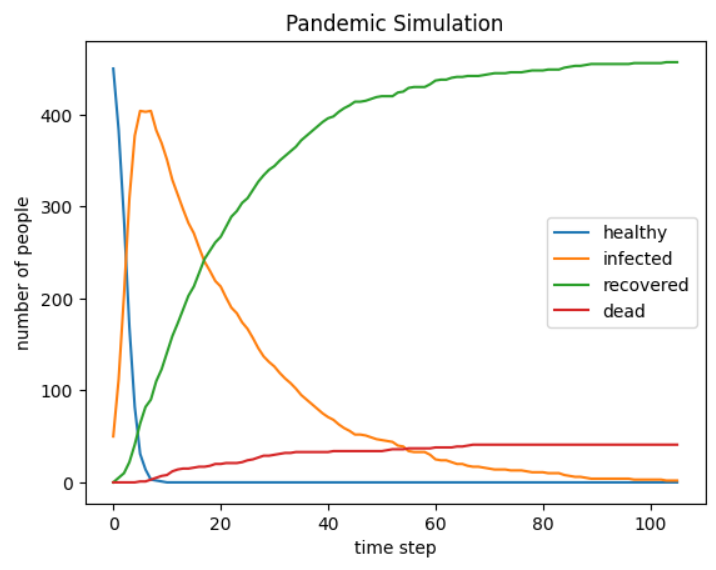
\includegraphics[width=.6\linewidth]{situation6.PNG}
    \caption{23 * 23 board with 500 people, (10\% infected), 105 time steps}
    \label{fig:enter-label}
\end{figure}
We ensure that our model is functioning correctly in this extreme case. The 23x23 board size was chosen specifically because it was the smallest square board which would allow 500 people on it without overlap. The results of the graph reflect this, with the disease spreading extremely quickly and the infection rate plateauing almost instantly. Since the death rate's randomizer does not depend on the size of the board, the death rate is the least affected by this change of parameters. \\\\
Finally, we have attached two gifs to the docs folder, which are named \href{https://github.com/UChi-ComPy23/group-project-group2/blob/main/doc/checkpoint/simulation1.gif}{Simulation 1} and \href{https://github.com/UChi-ComPy23/group-project-group2/blob/main/doc/checkpoint/simulation2.gif}{Simulation 2}. Simulation1.gif is for an 100x100 board shape, 100 time steps, 500 people, and 0.1\% initial infection, while Simulation2.gif is exactly the same except with a 50x50 board. As we can see from observing the gifs, they work correctly. In the second gif, the infection rate is much faster and so too is the recovery rate. This is because, in a much more condensed space, the disease will propagate much faster and herd immunity will arise quicker. This is represented in the gif as the blue (healthy) circles turning orange (infected) when they come into close proximity with another orange circle. They then turn green to signify that they recovered or red to signify that they died. One can also infer that the red dots are dead as a result of them no longer moving. The colors of the circles correspond exactly with the colors denoted on the legend of the plots.\\ 

\section{Additional Implementations }

\subsection{One improvement that will be made is the full implementation of the mask to add realism to our model.}

\subsubsection{Crucial Questions} One question we hope to answer is whether we can find any patterns or convergence in our method when running for very high numbers of time steps. To answer this, we plan on running multiple trials with different time steps. We will run n trials per amount of time steps to account for the error caused by the random nature of our model. This is an extremely important question within the context of a disease model. Convergence could imply that the population has sufficiently placated the disease or that herd immunity has been achieved. Therefore, we want to test both the nature and speed of convergence by implementing extra parameters such as the mask. By doing this, we can test how much masks speed up the placation of the disease. \\
\subsubsection{Changes to Code} For each person in the person class, we have implemented a self.mask in the initialization and have set this to 0 as a default. If the person is wearing a mask, self.mask=1. If so, while they are susceptible, they have a chance to completely avoid infection during this time step. This has already been implemented, but we will next implement the distribution of masks as a response to the pandemic. \\
\subsubsection{Data Obtaining} We have already used data on the effectiveness of masks from “Study Shows Probability of Getting Covid for Mask Wearers vs. Non-Mask Wearers.” by Bhavana Kunkalikar. Using data from this source, we decided that a person with a mask will have an 87 percent chance of avoiding infection during the susceptible phase. We plan on using additional data about the rate at which the general public decides to wear a mask as a response to disease. \\\\

\subsection{The next improvement we make will be the implementation of interpolation methods to approximate a function for the data which we plot.}
\subsubsection{Crucial Questions} The main question we want to answer from our model is how our data converges over long periods of time. Currently, we are plotting the number of people who are healthy, dead, recovered, and infected. By approximating each of these four lines as functions, we could plot the output of these functions as opposed to running our model for longer. This would let us approximate how our model would run for extremely long periods of time without ever actually having to run it for that amount of time steps. This would be extremely helpful for approximating convergence and would improve the performance of our process overall. \\
\subsubsection{Changes to Code} In order to make our plot, our code already implements a list that records the number of people healthy, sick, dead, and recovered at each time step. From this point, we would only need to interpolate this data and plot it separately from our main plot. We plan on testing multiple different interpolation methods (such as Legendre, Cholesky, etc), and examine these plots to see which gives the most reasonable interpretation of the data. \\
\subsubsection{Data Obtaining} For this change, we will not need to use outside data or models since we have learned these interpolation techniques in class. However, we will use relevant packages such as interp1d and Barycentric Interpolator. We do not plan on needing concepts from websites or papers for this particular change. \\\\
\subsection{We also plan on implementing a feature in which previously recovered people can become infected again.}
\subsubsection{Crucial Questions} In order to be an insightful model, we must not only test convergence with default parameters, but we must also do the same tests with other conditions. This way, we can compare how a population will react to a virus given multiple different starting conditions. One crucial condition, which could greatly affect the convergence of our model, is whether or not people can be infected more than once. If so, then it is possible that the number of people infected and recovered will no longer converge because these functions will no longer be monotone. In the present version of our code, people cannot be infected more than once, thus the number of people recovered will always be monotone increasing. However, if they can be infected more than once, the amount of people recovered might oscillate and may never converge. \\
\subsubsection{Changes to Code} This implementation will require many changes to the simulation class. The foremost among these changes will be to allow people who have recovered to be infected once again. This could either be done by this method or could be done by moving people to the healthy group as opposed to the recovered group after infection. \\
\subsubsection{Data Obtaining} For this change, we will be altering strictly our own code, so external data will likely not be needed for this. \\

\section{References}
Kunkalikar, Bhavana. “Study Shows Probability of Getting Covid for Mask Wearers vs. Non-Mask Wearers.” Https://Www.News-Medical.Net/, 4 Aug. 2022, www.news-medical.net/news/20220802/Study-shows-probability-of-getting-COVID-for-mask-wearers-vs-non-mask-wearers.aspx.

\end{document}